\chapter{Szczegóły implementacyjne symulacji}
\label{cha:symulacja}

\section{Wybór technologii}

Do wykonania symulacji zdecydowano się na wykorzystanie technologii przeglądarkowych. Obecnie, aplikacje działające w obrębie przeglądarki internetowej, są bardzo dynamicznie rozwijającym się obszarem inżynierii oprogramowania. Dzięki temu dostępna jest duża liczba narzędzi i bibliotek pozwalających na tworzenie aplikacji praktycznie dowolnego typu w tym właśnie symulacji oraz wizualizacji. Dodatkową zaletą aplikacji przeglądarkowych jest ich przenośność dzięki czemu możliwe jest ich uruchomienie na praktycznie każdym urządzeniu, które posiada zainstalowaną przeglądarkę internetową.
Poniżej opisano technologie na których przede wszystkim opiera się wykonana symulacja:

\subsection{Język programowania Typescript}

Jedynym językiem programowania wspieranym natywnie przez przeglądarki internetowe jest obecnie Javascript. Jednak dzięki odpowiednim narzędziom tzw. transpilerom jest możliwe pisanie kodu w innym języku a następnie przekształceniu go do języka Javascript.
W projekcie zdecydowano się na wykorzystanie języka Typescript. Jest to język stworzony przez firmę Microsoft i jest on transpilowany do języka Javascript. Posiada on składnię zbliżoną do języka Javascript dodatkowo jednak oferuje on przede wszystkim mechanizm statycznego typowania dzięki czemu możliwe jest wychwycenie błędów związanych z typami już na etapie kompilacji a nie jak w przypadku języków z dynamicznym typowaniem dopiero podczas działania aplikacji. W opinii autora aplikacji pozwoliło to na łatwiejszą pracę z kodem, zwiększenie jego czytelności oraz zmniejszając liczbę potencjalnych błędów.

\subsection{Biblioteka renderująca Pixi.js oraz WebGL}

Wizualizacja zachowania się stosu protokołów oraz przepływu pakietów wymaga efektywnego wyświetlania na ekranie skomplikowanej hierarchii wielu obiektów. W tym celu wykorzystano bibliotekę Pixi.js oferującą interfejs pozwalający na tworzenie hierarchii obiektów, dokonywanie przekształceń geometrycznych i rysowanie podstawowych obiektów graficznych takich jak linie, elipsy, wielokąty. Biblioteka wykorzystuje niskopoziomowe API dostarczane przez przeglądarkę o nazwie WebGL. WebGL pozwala na efektywne renderowanie grafiki dwu oraz trójwymiarowej bezpośrednio w przeglądarce i na wykorzystanie możliwości oferowanych przez nowoczesne karty graficzne.

\subsection{Tween.js - animacje}

Większość animacji wykonano przy wykorzystaniu techniki nazywanej jako ``inbetweening`` zaimplementowanej w bibliotece Tween.js. Technika polega na wykorzystaniu funkcji interpolującej w celu wygenerowania płynnego przejścia pomiędzy początkowym i końcowym stanem obiektu. 
Na przykładzie animacji polegającej na przesunięciu obiektu z jednej pozycji na inną technika ta generuje wszystkie pośrednie pozycje obiektu mając podaną pozycję początkową oraz końcową. Dodatkowo na charakter animacji wpływa funkcja użyta do interpolacji. Użycie funkcji liniowej powoduje, że obiekt porusza się ruchem jednostajnym i zatrzymuje się natychmiast w miejscu co nie wygląda naturalnie. Natomiast użycie funkcji sinusoidalnej lub kwadratowej daje znacznie bardziej realistyczne wrażenie, ponieważ obiekt stopniowo przyśpiesza a następnie zwalnia.

\section{Architektura aplikacji}

\begin{figure}[ht]
	\centerline{\frame{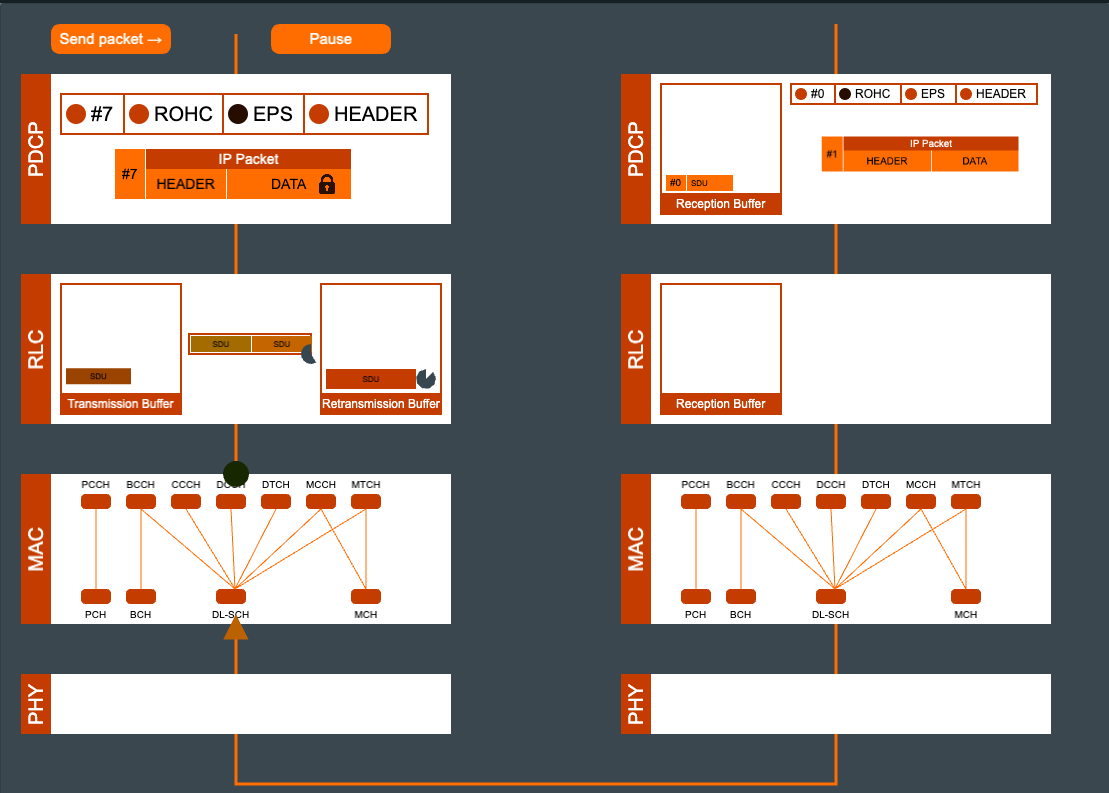
\includegraphics[width=0.8\textwidth]{images/simulation.png}}}
	\caption{Zrzut ekranu z wykonanej symulacji}
	\label{fig:simulation}
\end{figure}

Większość elementów widocznych na symulacji (Rys. \ref{fig:simulation}) została zaimplementowana jako osobne, niezależne obiekty. Każdy z obiektów zawiera logikę odpowiedzialną za jego wyświetlanie na ekranie jak i logikę odpowiedzialną za zamodelowanie odpowiadających mu mechanizmów związanych ze stosem protokołów LTE. Większość klas zaimplementowanych w ramach symulacji dziedziczy pośrednio lub bezpośrednio po klasie PIXI.Graphics dzięki czemu obiekty tej klasy mogą być renderowane, umieszczane w hierarchii obiektów a także mogą być na nich dokonywane transformacje geometryczne.

Poniżej opisano najbardziej kluczowe komponenty użyte w symulacji:

\subsection{Klasa Simulation}

Diagram UML dla klasy Simulation przedstawiono na Rys. \ref{fig:simulation_class}. Zawiera ona obiekty wszystkich symulowanych warstw, połączenia między nimi a także odpowiada za ich inicjalizację. Zawiera również obiekt klasy IPPacketGenerator odpowiadający za generowanie pakietów IP o losowej długości i inicjuje jego połączenie z przyciskiem ``Send packet``. Dzięki temu wciśnięcie przycisku powoduje wygenerowanie nowego pakietu IP i wysłanie go do pierwszej symulowanej podwarstwy tj. PDCP.

\begin{figure}[ht]
	\centerline{\frame{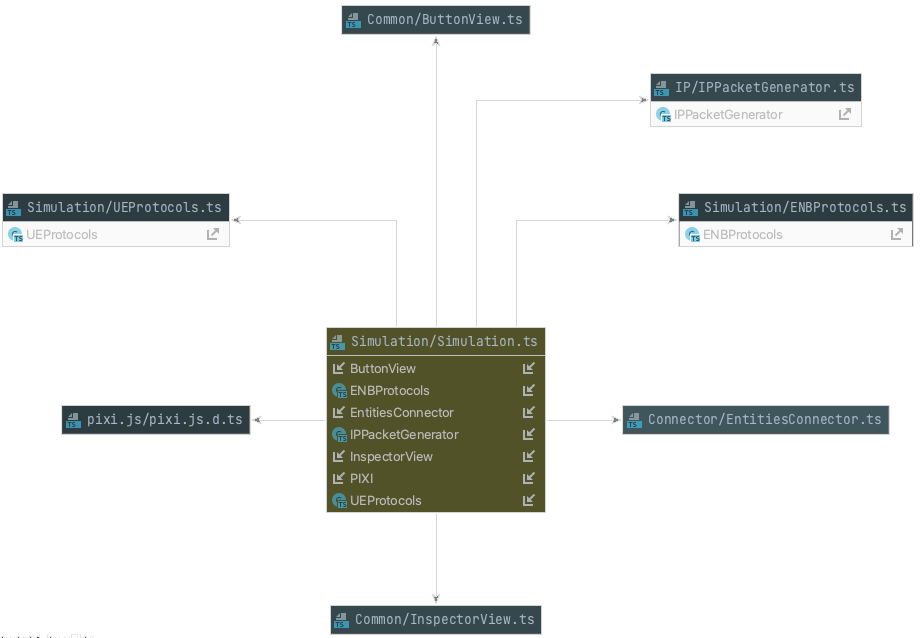
\includegraphics[width=0.9\textwidth]{images/simulation_class.png}}}
	\caption{Diagram UML dla klasy Simulation}
	\label{fig:simulation_class}
\end{figure}

\subsection{Klasa abstrakcyjna Connectable i interfejs DataUnit}

Najczęściej symulowanym zachowaniem w projekcie jest przesyłanie jednostek danych z jednego miejsca w drugie. Dlatego jednym z podstawowych komponentów, szeroko używanych w symulacji jest klasa abstrakcyjna Connectable. Posiada ona 2 kanały: A oraz B które umożliwiają przesyłanie w dwóch kierunkach obiektów implementujących interfejs DataUnit. Pozwala to na:

\begin{enumerate}
	\item wysyłanie jednostek danych do obiektu
	\item wysyłanie jednostek danych z obiektu do innych obiektów, które są podłączone do któregoś z kanałów danego obiektu
	\item łączenie obiektów razem ze sobą przy użyciu kanałów
	\item implementację dowolnej logiki reagowania na pojawienie się danych w kanale w klasach dziedziczących po klasie Connectable
\end{enumerate}

Domyślna reakcja obiektów dziedziczących po klasie Connectable na pojawienie się jednostki w kanale to przesłanie obiektu do drugiego kanału. Oznacza to, że obiekty wysłane do kanału A zostają odebrane a następnie opublikowane na kanale B. Natomiast obiekty wysłane do kanału B zostają opublikowane na kanale A. Dzięki temu domyślnie, obiekty dziedziczące po klasie Connectable, zachowują się jak przewodniki. Takie zachowanie można zaobserwować np. w komponentach łączących warstwy pomiędzy sobą. Natomiast klasy implementujące poszczególne warstwy nadpisują domyślne zachowanie poprzez dodanie logiki odpowiadającej za przetwarzanie odebranych jednostek danych, buforowanie ich czy dodawanie nagłówków przed przesłaniem dalej.

\begin{figure}[ht]
	\centerline{\frame{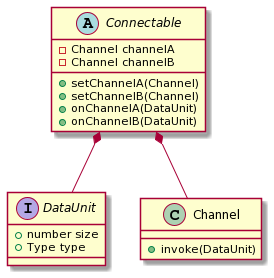
\includegraphics[width=0.3\textwidth]{images/connectable_class.png}}}
	\caption{Diagram UML dla klasy Connectable}
	\label{fig:connectable_class}
\end{figure}

\subsection{Klasa LayerView}

Implementuje części wspólne wszystkich podwarstw przedstawionych w symulacji. Tj. renderowanie nagłówka z nazwą podwarstwy oraz białego pola, gdzie przedstawione są mechanizmy wchodzące w skład podwarstwy. Rys. \ref{fig:layer_view_class}

\begin{figure}[ht]
	\centerline{\frame{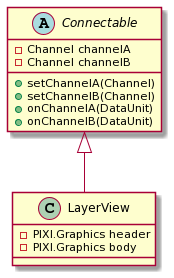
\includegraphics[width=0.2\textwidth]{images/layer_view_class.png}}}
	\caption{Diagram UML dla klasy LayerView}
	\label{fig:layer_view_class}
\end{figure}

\subsection{Klasa BufferView}

W kilku miejscach symulacji można zauważyć wizualizację buforów przechowujących jednostki danych. Ich zachowanie polega na dodawaniu i usuwaniu jednostek danych a także układaniu ich w odpowiedniej kolejności. Ta logika została zaimplementowana przy użyciu klasy BufferView (Rys. \ref{fig:buffer_view_class}).

\begin{figure}[ht]
	\centerline{\frame{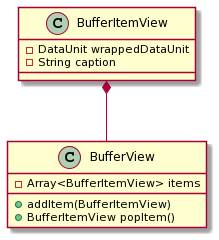
\includegraphics[width=0.2\textwidth]{images/buffer_view_class.png}}}
	\caption{Diagram UML dla klasy BufferView}
	\label{fig:buffer_view_class}
\end{figure}
